\documentclass[a4paper,10pt,reqno]{amsart}

\usepackage[utf8]{inputenc}
\usepackage[foot]{amsaddr}
\usepackage{amsmath,amsfonts,amssymb,amsthm,mathrsfs,bm}
\usepackage[margin=0.95in]{geometry}
\usepackage{color}
\usepackage[dvipsnames]{xcolor}

\input{toc-config.tex}

\usepackage{mathtools,enumerate,mathrsfs,graphicx}
\usepackage{epstopdf}
\usepackage{hyperref}

\usepackage{latexsym}


\definecolor{CommentGreen}{rgb}{0.0,0.4,0.0}
\definecolor{Background}{rgb}{0.9,1.0,0.85}
\definecolor{lrow}{rgb}{0.914,0.918,0.922}
\definecolor{drow}{rgb}{0.725,0.745,0.769}

\usepackage{listings}
\usepackage{textcomp}
\lstloadlanguages{Matlab}%
\lstset{
    language=Matlab,
    upquote=true, frame=single,
    basicstyle=\small\ttfamily,
    backgroundcolor=\color{Background},
    keywordstyle=[1]\color{blue}\bfseries,
    keywordstyle=[2]\color{purple},
    keywordstyle=[3]\color{black}\bfseries,
    identifierstyle=,
    commentstyle=\usefont{T1}{pcr}{m}{sl}\color{CommentGreen}\small,
    stringstyle=\color{purple},
    showstringspaces=false, tabsize=5,
    morekeywords={properties,methods,classdef},
    morekeywords=[2]{handle},
    morecomment=[l][\color{blue}]{...},
    numbers=none, firstnumber=1,
    numberstyle=\tiny\color{blue},
    stepnumber=1, xleftmargin=10pt, xrightmargin=10pt
}

\numberwithin{equation}{section}
\synctex=1

\hypersetup{
    unicode=false, pdftoolbar=true, 
    pdfmenubar=true, pdffitwindow=false, pdfstartview={FitH}, 
    pdftitle={ELE2024 Coursework}, pdfauthor={A. Author},
    pdfsubject={ELE2024 coursework}, pdfcreator={A. Author},
    pdfproducer={ELE2024}, pdfnewwindow=true,
    colorlinks=true, linkcolor=red,
    citecolor=blue, filecolor=magenta, urlcolor=cyan
}


% CUSTOM COMMANDS
\renewcommand{\Re}{\mathbf{re}}
\renewcommand{\Im}{\mathbf{im}}
\newcommand{\R}{\mathbb{R}}
\newcommand{\N}{\mathbb{N}}
\newcommand{\C}{\mathbb{C}}
\newcommand{\lap}{\mathscr{L}}
\newcommand{\dd}{\mathrm{d}}
\newcommand{\smallmat}[1]{\left[ \begin{smallmatrix}#1 \end{smallmatrix} \right]}

%opening
\title[ELE2024 Coursework]{ELE2024 coursework - Group 1}

\author[O. McCullough]{Owen McCullough}
\author[O. Quail]{Orla Quail}
\author[E. Acton]{Eoin Acton}

\begin{document}

\maketitle

\section*{Introduction}
The aim of this report is to design a controller for a system of a wooden ball on an inclined plane, with a spring and damper, where the ball can be attracted downwards by an electromagnet.
A labelled diagram of the system is shown in \hyperref[fig:system]{Figure 1}.

\begin{figure}[h]
\centering
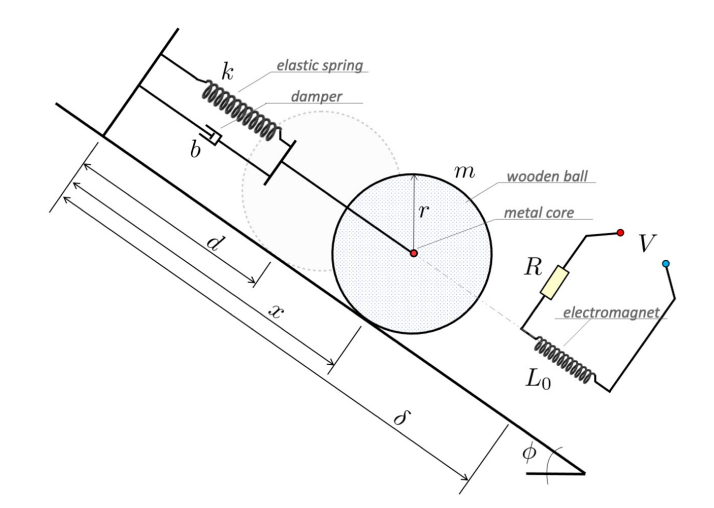
\includegraphics[width=0.6\linewidth]{ControlCW_sys_diagram.png}
\caption{Wooden ball on an incline plane. The ball can be attracted towards an electromagnet through controlling a voltage $V$}
\label{fig:system}
\end{figure}

\section{Modelling}
From \hyperref[fig:system]{Figure 1}, we can define the total force acting on the ball as:
\begin{equation}
\label{eq:total_F}
    F_{total}=F_{magnet}+F_{ball}-F_{spring}-F_{dampener}
\end{equation}

\subsection{Spring and dampener}
Hooke's law states that the restoring force exerted by a spring is proportional to the displacement (or deformation) and opposite in
direction. Therefore, the spring and dampener forces are modelled in the following equations:
\begin{subequations}
\label{eq:spring_dampener}
\begin{align}
    F_{spring}&=k(x-d), \\
    F_{dampener}&=b\dot x
\end{align}
\end{subequations}

Where $k$ is the stiffness of the spring, equal to $1885 N/m$, and $b$ is the viscous damping coefficient, equal to $10.4 Ns/m$, while $x$ and $d$ are distances shown in \hyperref[fig:system]{Figure 1}.

\subsection{The Wooden Ball}
The force of gravity acting on the ball can be written as:
\begin{equation*}
\label{eq:grav}
    F_{gravity}=mg
\end{equation*}
where $m$ is the mass of the ball, equal to $462g$, and $g$ is the gravitational constant, equal to $9.81m/s^2$. Due to the inclined plane, the force must be split into horizontal and vertical components:
\begin{equation*}
\label{eq:grav_resolved}
    F_{gravity}=mg\cos{\phi}+mg\sin{\phi}
\end{equation*}
In \hyperref[fig:system]{Figure 1}, from the reference frame of the incline plane, we observe that the ball cannot move vertically downwards, therefore the vertical component of $F_{gravity}$, $mg\cos{\phi}$ will be equal to 0:
\begin{equation*}
\label{eq:grav_sin}
    F_{gravity}=mg\sin{\phi}
\end{equation*}
In the problem statement provided, it was stated that the ball can move without slipping. This means there is a secondary force $T$ acting on the ball from the point of contact with the incline plane. Combining this force with $F_{gravity}$, we can begin solving for an equation of motion:
\begin{equation}
\label{eq:ball_1}
    F_{ball}=mg\sin{\phi}-T=ma=m\ddot x
\end{equation}
The equation for the force $T$, can be written as:
\begin{equation*}
\label{eq:torque_1}
    T=\frac{M}{r}
\end{equation*}
Where $M$ is the torque and $r$ is the radius of the wooden ball from \hyperref[fig:system]{Figure 1}. As the torque is defined as the moment of inertia $I$ multiplied by the angular acceleration $\ddot \theta$, the following equation can be written:
\begin{equation}
\label{eq:torque_2}
    T=\frac{I\ddot \theta}{r}
\end{equation}
Using the arc-length theorem, we can derive the following identity for $\ddot x$:
\begin{equation*}
    x=r\theta
\end{equation*}
Therefore:
\begin{equation}
\label{eq:arc-len-dir}
    \ddot x=r\ddot \theta
\end{equation}
Combining the above equation for $T$ \eqref{eq:torque_2} with \eqref{eq:ball_1} results in the equations below:
\begin{gather*}
    \notag mg\sin{\phi}-\frac{I\ddot \theta}{r}=ma=m\ddot x, \\
    \notag mg\sin{\phi}=(\frac{I}{r}+mr)\ddot \theta, \\
\end{gather*}  
Then, substituting the equation for moment of inertial for a sphere as well as the identity established in (\ref{eq:arc-len-dir}) results in the equations below:
\begin{align*}
    \notag mg\sin{\phi}&=(\frac{2}{5}+1)mr\ddot \theta, \\
    \notag mg\sin{\phi}&=\frac{7}{5}m\ddot x, \\
\end{align*}
Therefore:
\begin{equation}
\label{eq:ball_2}
      F_{ball}=g\sin{\phi}-\frac{7}{5}\ddot x
\end{equation}

\subsection{Electromagnet}
In the provided problem statement, $F_{magnet}$ was defined as:
\begin{equation}
\label{eq:mag}
    F_{magnet}=c^2\frac{i^2}{y^2}
\end{equation}
where $i$ is the current that runs through the circuit, $y=(\delta-x)$, and $c$ is a positive constant equal to $6.811 \frac{m^3g}{A^2s^2}$. 

The current $i$ can be derived using Kirchoff's Voltage Law (KVL) which states that the directed sum of the voltages around any
closed loop is zero.
Using this theorem, the following equation can be derived:
\begin{equation}
\label{eq:circuit}
    V= iR + L\dot{i}
\end{equation}
Where L is given as $L = L_0 + L_1exp(-\alpha y)$, and resistance $R$ is equal to $2.2 k \Omega$.

Therefore, rearranging \eqref{eq:circuit} and substituting in for $L$, allows the following equation to be obtained:
\begin{equation}
\label{eq:I_dot}
    \dot{i} = \frac{V-iR}{L_0 + L_1e^{(-\alpha y)}}
\end{equation}

\subsection{State Space Representation}
Combining the force equations \eqref{eq:total_F}, \eqref{eq:spring_dampener} \eqref{eq:ball_2} and \eqref{eq:mag} allows the following equation to be derived:
\begin{equation}
\label{eq:unlinear_model}
    \frac{7}{5}m\ddot x=c\frac{i^2}{(\delta-x)^2}+mg\sin{\phi}-k(x-d)-b\dot x
\end{equation}
To obtain SSR, three new variables are created:
\begin{align*}
x_1&=x, \\
x_2&=\dot x, \\
x_3&=i
\end{align*}
Substituting these new variables into \eqref{eq:unlinear_model} allows the following SSR to be obtained:
\begin{equation}
\label{eq:SSR}
    \mathbf{\dot x} = f(\mathbf x, V) = \begin{bmatrix} 
        \dot x_1 \\ 
        \dot x_2 \\ 
        \dot x_3 
    \end{bmatrix} = \begin{bmatrix}
        x_2 \\
        \frac{5}{7m}(c\frac{{x_3}^2}{(\delta-x_1)^2}+mg\sin{\phi}-k(x_1-d)-bx_2) \\
        \frac{V-x_3R}{L_0+L_1e^{-\alpha(-\delta-x_1)}}
    \end{bmatrix}
\end{equation}


\section{Linearisation of System Equations}
The definitions for the dynamical system derived in \eqref{eq:SSR} can be written as:
\begin{align}
\notag \dot x_1 &= x_2,                  \\
\notag \dot x_2 &= \theta(x_1, x_2, x_3),  \\
\notag \dot x_3 &= \psi(V, x_1, x_3)
\end{align}
Where the functions $\theta(x_1, x_2, x_3)$ and $\psi(V, x_1, x_3)$ represent the acceleration of the ball and the rate of change of the current in the electromagnet respectively.
To obtain a linear approximation for $\theta(x_1, x_2, x_3)$ and $\psi(V, x_1, x_3)$ around the equilibrium points $(x_1^e, x_2^e, x_3^e, V^e)$, the following partial derivatives can be derived for both functions:
\begin{subequations}
\label{eq:theta__psi_constants}
\begin{align}
    A = \frac{\partial \theta(x_1,x_2,x_3)}{\partial x_1}\bigg|_{x_1^e, x_2^e, x_3^e} &= \frac{5 \cdot \left(\frac{2 c {x_{3}^e}^{2}}{\left(\delta - x_{1}^e\right)^{3}} - k\right)}{7 m}, \\
    B = \frac{\partial \theta(x_1,x_2,x_3)}{\partial x_2}\bigg|_{x_1^e, x_2^e, x_3^e} &= - \frac{5 b}{7 m}, \\
    C = \frac{\partial \theta(x_1,x_2,x_3)}{\partial x_3}\bigg|_{x_1^e, x_2^e, x_3^e} &= \frac{10 c x_3^e}{7 m \left(\delta - x_1^e\right)^{2}}
\end{align}
and
\begin{align}
    D = \frac{\partial \psi(V,x_1,x_3)}{\partial x_1}\bigg|_{V^e, x_1^e, x_3^e} &= - \frac{L_{1} \alpha \left(- R x_{3}^e + V\right) e^{- \alpha \left(\delta - x_{1}^e\right)}}{\left(L_{0} + L_{1} e^{- \alpha \left(\delta - x_{1}^e\right)}\right)^{2}}, \\
    E = \frac{\partial \psi(V,x_1,x_3)}{\partial x_3}\bigg|_{V^e, x_1^e, x_3^e} &=- \frac{R}{L_{0} + L_{1} e^{- \alpha \left(\delta - x_{1}^e\right)}}, \\
    F = \frac{\partial \psi(V,x_1,x_3)}{\partial V}\bigg|_{V^e, x_1^e, x_3^e} &=\frac{1}{L_{0} + L_{1} e^{- \alpha \left(\delta - x_{1}^e\right)}}
\end{align}
\end{subequations}
According to Taylor's Theorem:
\begin{equation}
\label{eq:taylor_theorem}
    \phi(x) \approx \phi(x_0) + \phi'(x_0)(x-x_0).
\end{equation}
From Taylor's theorem, the following approximation for $\theta(x_1, x_2, x_3)$ can be derived:
\begin{equation}
\label{eq:taylor_theta_applied}
    \theta \approx \theta^{e} + A(x_1-x_1^e) + B(x_2-x_2^e) + C(x_3-x_3^e)
\end{equation}
Similarly, for $\psi(V, x_1, x_3)$:
\begin{equation}
\label{eq:taylor_psi_applied}
    \psi \approx \psi^{e} + D(x_1-x_1^e) + E(x_3-x_3^e) + F(V-V^e)
\end{equation}
In order to remove constant terms for the system, deviation variables need to be introduced. For this system, the deviation variables are defined as $\bar x_1=(x_1-x_1^e)$, $\bar x_2=(x_2-x_2^e)$, $\bar x_3=(x_3-x_3^e)$, and $\bar V=(V-V^e)$. Therefore, the equations \eqref{eq:taylor_theta_applied} and \eqref{eq:taylor_psi_applied} can be rewritten by substituting in the deviation variables  $\bar x_1$, $\bar x_2$, $\bar x_3$ and $\bar V$:
\begin{align}
\label{eq:taylor_dev}
    \theta &\approx \theta^e + A\bar x_1 + B\bar x_2 + C\bar x_3, \\
    \psi &\approx \psi^e + D\bar x_1 + E\bar x_3 + F\bar V
\end{align}
Therefore, the SSR \eqref{eq:SSR} obtained in the previous section can now be rewritten in the following linear form:
\begin{equation}
\label{eq:SSR_lin}
    \mathbf{\dot \bar{x}} = f(\mathbf x, V) = \begin{bmatrix} 
        \dot x_1 \\ 
        \dot x_2 \\ 
        \dot x_3 
    \end{bmatrix} \approx \begin{bmatrix}
        x_2 \\
        A\bar x_1 + B\bar x_2 + C\bar x_3 \\
        D\bar x_1 + E\bar x_3 + F\bar V
    \end{bmatrix}
\end{equation}
$\theta^e$ and $\psi^e$ have been omitted as they are equal to 0 at their equilibrium points.

\subsection{Determining Equilibrium Points} In order to determine equilibrium points, it is necessary to set $f(\mathbf x, V)=0$:
\begin{equation}
\label{eq:ssr_eq_points_1}
    f(\mathbf{x^e}, V^e) = \begin{bmatrix} 
        \dot x_1^e \\ 
        \dot x_2^e \\ 
        \dot x_3^e 
    \end{bmatrix} = \begin{bmatrix}
        x_2 \\
        \frac{5}{7m}(c\frac{{x_3^e}^2}{(\delta-x_1^e)^2}+mg\sin{\phi}-k(x_1^e-d)-bx_2^e) \\
        \frac{V-x_3^eR}{L_0+L_1\exp{-\alpha(-\delta-x_1^e)}}
    \end{bmatrix} = \begin{bmatrix}
        0 \\
        0 \\
        0
    \end{bmatrix}
\end{equation}
From equation \eqref{eq:ssr_eq_points_1}, a set of of state variables $\mathbf{x^e}$ and an input voltage $V^e$ are defined. The aim of the controller is to maintain a position of 0.5m for the ball, therefore, the value of 0.5 m can be used as the equilibrium point for $x_1$, hence $x_1^e=0.5$ m. The equilibrium points $x_2^e$, $x_3^e$, and $V^e$ can then be determined algebraically. Using the Python module sympy, we obtained the following values for $\mathbf{x^e}$ and $V^e$:
\begin{equation}
    \mathbf{x^e} = \begin{bmatrix}
        x_1^e \\
        x_2^e \\
        x_3^e
    \end{bmatrix} = \begin{bmatrix}
        0.5m \\
        0ms^-1 \\
        22.373A
    \end{bmatrix}
\end{equation}
\begin{align}
    V^e = 49220.035V
\end{align}


\section{Controller Design}
\subsection{Defining a Transfer Function} 
The transfer function is an expression of the output of a given system against an input to the system, where it is assumed the initial conditions are zero. The transfer function is important as it allows simulation of the system response for different inputs in order to create a comprehensive control system that returns the system state to the equilibrium point for a wide range of inputs. The transfer function is defined below
\begin{align}
G(s) = \frac{X(s)}{U(s)}
\end{align}
where $x$ and $u$ denote the input and state of a linear dynamical system, and $X(s)$ and $U(s)$ denote their corresponding Laplace transforms.
\\ \\
The relevant output variable to be studied within this report is the position of the wooden ball $x_1$. Therefore, a transfer function with output variable $\bar{X_1}(s)$  and input variable $\bar{V}(s)$ needs to be derived. $G_x$ is used to denote this transfer function, as shown in \eqref{eq:G_x}.
\begin{equation}
    \label{eq:G_x}
    G_x(s)=\frac{\bar X_1(s)}{\bar V(s)}
\end{equation}

The Laplace transform of the linear approximation of the system obtained in \eqref{eq:SSR_lin} is shown below.
\begin{align*}
    \lap\{\dot x_1(t)\} &= s\bar X_1(s) = X_2(s) \\
    \lap\{\dot x_2(t)\} &= s\bar X_2(s) = A\bar X_1(s)+B\bar X_2(s)+C\bar X_3(s) \\
    \lap\{\dot x_3(t)\} &= s\bar X_3(s) = D\bar X_1(s)+E\bar X_3(s)+F\bar V(s) \\
\end{align*}

The derivation for the transfer function $G_x$ can be seen below:
\begin{align}
\label{eq:G_x_1}
    \notag s\bar X_3(s) &= D\bar X_1(s) + E\bar X_3(s)+F\bar V(s) \\
    \notag F\bar V(s) + D\bar X_1(s) &= s\bar X_3(s)-E\bar X_3(s) \\
    \notag F\bar V(s) + D\bar X_1(s) &= (s-E)\bar X_3(s) \\
    \bar X_3(s)&=\frac{F\bar V(s) + D\bar X_1(s)}{s-E}
\end{align}
\begin{align}
\label{eq:G_x_2}
    \notag s\bar X_2(s) &= A\bar X_1(s)+B\bar X_2(s)+C\bar X_3(s) \\
    \notag s(s\bar X_1(s)) &= A\bar X_1(s)+B(s\bar X_1(s))+C\bar X_3(s) \\
    \notag s^2\bar X_1(s) &= A\bar X_1(s)+sB\bar X_1(s)+C\bar X_3(s) \\
    \notag C\bar X_3(s) &= s^2\bar X_1(s)-A\bar X_1(s)-sB\bar X_1(s) \\
    C\bar X_3(s) &= \bar X_1(s)(s^2-sB-A)
\end{align}
Substituting equation \eqref{eq:G_x_1} into equation \eqref{eq:G_x_2} gives:
\begin{align}
    \notag C(\frac{F\bar V(s) + D\bar X_1(s)}{s-E}) &= \bar X_1(s)(s^2-sB-A) \\
    \notag CF\bar V(s) + CD\bar X_1(s) &= (s-E)(s^2\bar X_1(s)-A\bar X_1(s)-sB\bar X_1(s)) \\
    \notag CF\bar V(s) &= \bar X_1(s)(s^3 +s^2(B-E) +s(-BE-A) +AE -CD) \\
    \notag \frac{\bar X_1(s)}{\bar V(s)} &= \frac{CF}{(s^3 +s^2(-B-E) +s(BE-A) +AE -CD)}\\
\end{align}

Therefore, the transfer function $G_x$ can be defined as
\begin{equation}
    G_x = \frac{CF}{(s^3 +s^2(-B-E) +s(BE-A) +AE -CD)}\\
\end{equation}

\subsection{BIBO Stability}
A dynamical system with input $u$ and output $x$ is called BIBO stable if its output is bounded whenever its input is bounded. Mathematically, it is defined as the impulse response of a system's transfer function $G(s)$ being absolutely integral:
\begin{equation*}
    \int_{0}^{\infty} \lap^{-1}\{G(s)\}(\tau)d\tau < \infty
\end{equation*}
Where $\lap^{-1}\{G(s)\}(\tau)$ is the impulse response of a transfer function in the time-domain. Checking for BIBO stability of a system is important as it allows the long term effect of an input on the system output to be observed.
\\ \\ 
The impulse response of our transfer function $G_x(s)$ can be seen below in \hyperref[fig:no-pid-impulse]{Figure 2}.

\begin{figure}[h]
\centering
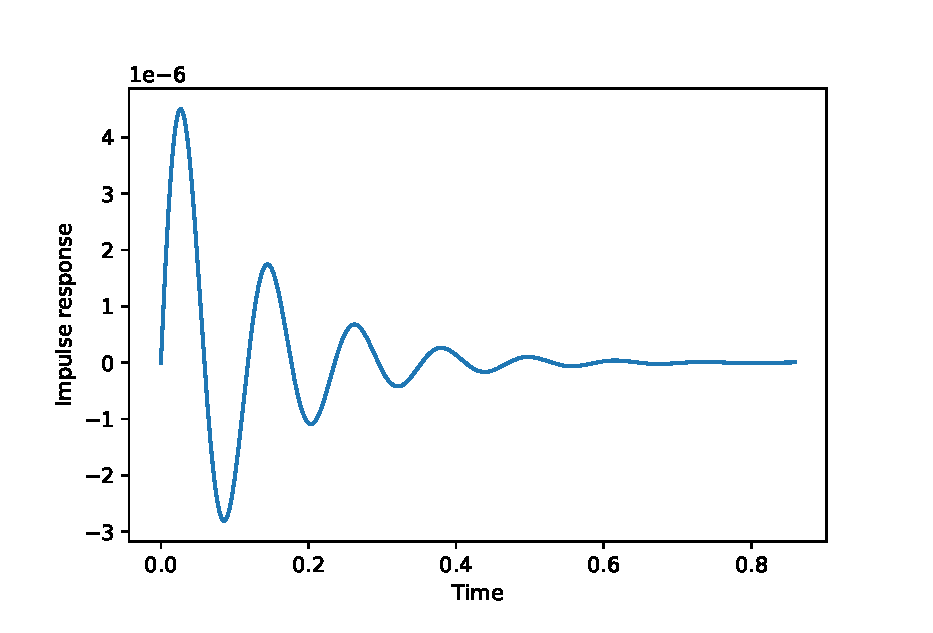
\includegraphics[width=0.6\linewidth]{g-x-impulse.eps}
\caption{The impulse response of $G_x$}
\label{fig:no-pid-impulse}
\end{figure}
\hyperref[fig:no-pid-impulse]{Figure 2} shows that $G_x$ is absolutely integrable as it converges to 0, therefore, $G_x$ is BIBO stable.

\subsection{Sensor Design}
The position of the ball is measured with a sensor that can be modelled as a first-order system. The derivation of the transfer function for the sensor can be seen below:
\begin{equation}
\label{eq:sensor_1}
    x(t)+\tau_m\dot x(t)=K_mu(t)
\end{equation}
In order to derive the transfer function, the Laplace transform must be applied to Equation \eqref{eq:sensor_1}.
\begin{align*}
    X(s)+\tau_msX(s)=K_mU(s) \\
    X(s)(1+\tau_ms)=K_mU(s)
\end{align*}
The transfer function for the sensor $G_s(s)$ can then be defined as:
\begin{equation}
    \frac{X(s)}{U(s)}=\frac{K_m}{1+\tau_ms}
\end{equation}

The time constant $\tau_m$ is equal to 30ms. The value of the static gain $K_m$ was chosen to be $1$ to ensure that the output of the sensor accurately reflects the position of the ball. \\ \\ 
The sensor acts as a 30ms delay between the output of the system and the PID controller to emulate the effects a sensor would have on a practical system with the same design. 


\subsection{Designing a PID Controller}
PID controllers are defined by the following equation:
\begin{align}
    u(t) = K_pe(t) + K_d\dot{e}(t) + K_iI(t)
\end{align}
where $u(t)$ is the output of the system, $e(t)$ is the control error (deviation from the set point), $K_p$ is the proportional gain value, $K_d$ is the derivative gain value, $I(t)$ is the time-integral of the error and $K_i$ is the integral gain value. When $u(t) = 0$, the system is at the set point.
\\ \\ 
Increasing $K_p$ allows the controller to react to the error faster. However, if the $K_p$ value is too large, this may lead to oscillations and may leave the controller unable to converge the system to the set point.
\\ \\
The derivative gain $K_d$ is used to suppress the oscillations created by the $K_p$ and therefore allow the system to converge to the set point.
\\ \\
Often, the model of the system is too simple and doesn't account for many other variables that in reality the system would face. Therefore, there is often a difference between the set point and the limit of the system output, this is called offset. Offset is eliminated by $K_i$.
\\ \\
In order to design an appropriate PID controller for this system, we defined the following constraints our controller should meet:
\begin{itemize}
    \item The system should not have any major oscillations
    \item The system should not oscillate greater than $\pm 5$mm around the set point
    \item The system should converge to its set point within 1.5 seconds
\end{itemize}

After we decided on our criteria that our PID controlled system must have, we developed a PID controller with the following values:
\begin{align*}
\label{PID values}
    K_p &= 980 \\
    K_i &= 1 \\
    K_d &= 10
\end{align*}

The PID controller is then connected in series with the system's transfer function $G_x(s)$, with the sensor's transfer function $G_s(s)$ in a feedback loop across that series connection. The entire closed loop system's transfer function is defined as:
\begin{equation}
    G_{cl}(s)=\frac{G_s(s)}{1+G_s(s)G_c(s)G_x(s)}
\end{equation}
The impulse and step responses of the closed loop system can be seen below in \hyperref[fig:pid-impulse]{Figure 3} and \hyperref[fig:pid-step]{Figure 4} respectively.
\begin{figure}[h]
\centering
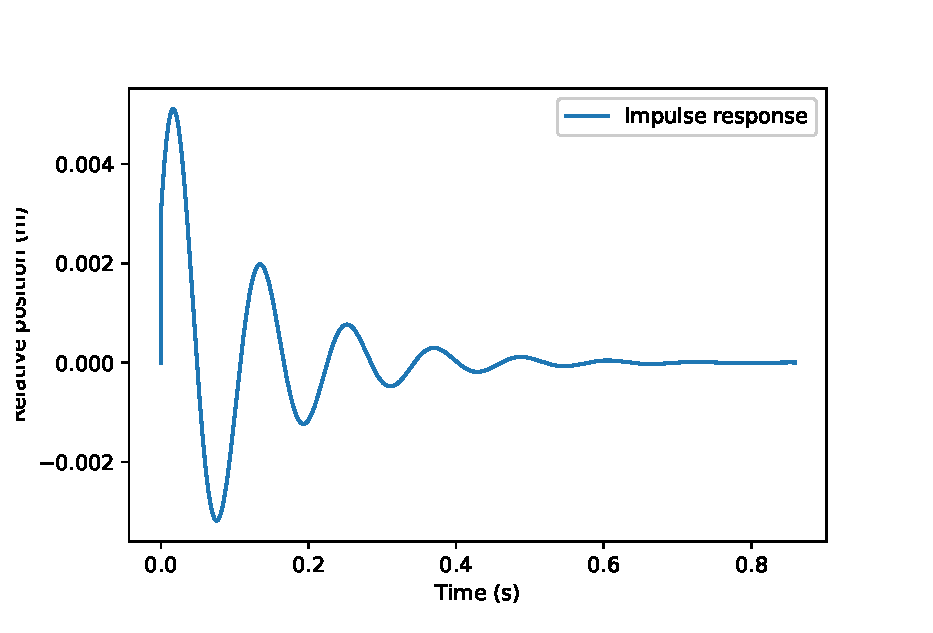
\includegraphics[width=0.6\linewidth]{g-load-impulse.eps}
\caption{Impulse response of the closed loop system $G_{cl}(s)$}
\label{fig:pid-impulse}
\end{figure}
\begin{figure}[!h]
\centering
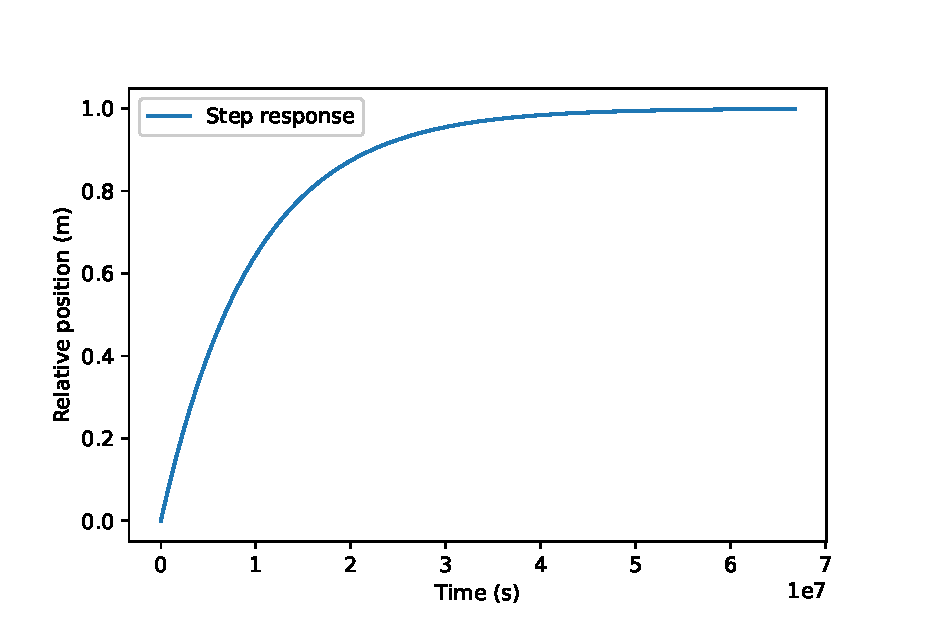
\includegraphics[width=0.6\linewidth]{g-load-step.eps}
\caption{Step response of the closed loop system $G_{cl}(s)$}
\label{fig:pid-step}
\end{figure}


%The closed loop transfer function of the system after the sensor and PI controller have been added is:
%\begin{equation}
%    \label{eq:Gload4}
%    G_{cl}(s) = \frac{4.329s^2 + 144.3s}{0.03s^5 + 456.2s^4 + 1.484\cdot 10^5s^2 + 1.159 \cdot 10^6 s + 1.443 \cdot 10^{-6}}
%\end{equation}

\subsection{Routh's Stability Criterion}
Routh's tabulation is a method that can be used to test for BIBO stability, as it can be used to tell whether a given polynomial has any roots with a non-negative real part. The number of roots with a positive real part is equal to the number of sign changes in the first column of Routh's tabulation. A system is only BIBO stable if all poles of a given polynomial have a negative real part.
\begin{equation}
G_{cl}(s)=\frac{1.369 s^3 + 179.8 s^2 + 4472 s + 4.563}{0.03 s^5 + 456.2 s^4 + 2.257 \times 10^{4} s^3 + 1.571 \times 10^{6} s^2 + 4.414 \times 10^{7} s + 4.563}
\label{eq:g-load-subbed}    
\end{equation}
Given Equation \eqref{eq:g-load-subbed}, Routh's tabulation for the characteristic polynomial of $G_{cl}$, $Q(s) = 0.03s^5 + 456.2s^4 + 2.257\cdot 10^4s^3 + 1.571 \cdot 10^6s^2 + 4.414 \cdot 10^7s + 4.563$, dictates that there are no sign changes in the first column and none of the coefficients of $s$ are equal to $0$. Therefore, all poles of the polynomial have a negative real part, and the closed loop transfer function $G_{cl}$ is BIBO stable.

\section{Disturbance Rejection} To ensure that our system can handle disturbances, we needed to make sure that our system with another input $D(s)$ is still BIBO stable and has zero offset when encountering a step-input from $D(s)$. The disturbance input $D(s)$ will act on the system output through a transfer function $G_d(s)$ which is equivalent to our system transfer function $G_x(s)$. First, we assume our original input $\bar V(s)=0$, then we can derive a new transfer function for disturbances:
\begin{gather}
    \notag \bar X_1 = (\bar V(s)-\bar X_1(s)G_s(s))G_x(s)G_c(s)+D(s)G_d(s) \\
    \notag \bar X_1 = G_x(s)G_c(s)\bar V(s) - G_x(s)G_c(s)G_s(s)\bar X_1(s) + D(s)G_d(s) \\
    \notag \bar X_1 = -G_x(s)G_c(s)G_s(s)\bar X_1(s) + D(s)G_d(s) \\
    \notag D(s)G_d(s) = \bar X_1(s) + G_x(s)G_c(s)G_s(s)\bar X_1(s) \\
    \notag D(s)G_d(s) = \bar X_1(s)(1 + G_x(s)G_c(s)G_s(s))
\end{gather}
To observe the response of our system to changes in disturbances, we define our closed-loop transfer function as:
\begin{equation*}
    G(s)=\frac{\bar X_1(s)}{D(s)}
\end{equation*}
Therefore:
\begin{equation}
\label{eq:dist-transfer}
    G(s)=\frac{\bar X_1(s)}{D(s)}=\frac{G_d(s)}{1 + G_x(s)G_c(s)G_s(s)}
\end{equation}
\hyperref[fig:dist-step]{Figure 5} shows the response of the transfer function from (\ref{eq:dist-transfer}) to step change in input.
\begin{figure}[!h]
\centering
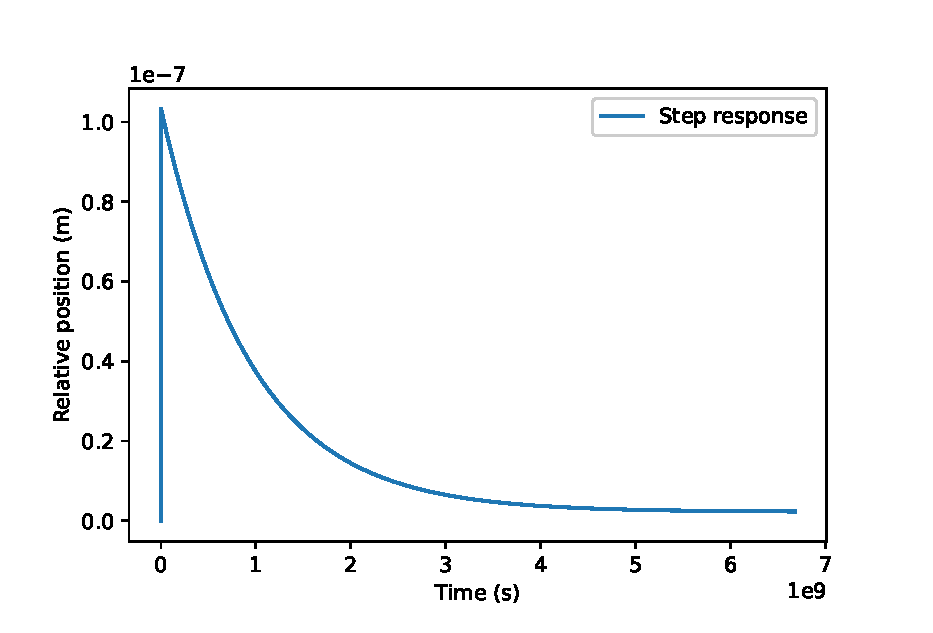
\includegraphics[width=0.6\linewidth]{g-load-disturbance-rejection.eps}
\caption{Disturbance step response of the closed loop system $G_{cl}(s)$}
\label{fig:dist-step}
\end{figure}
\hyperref[fig:dist-imp]{Figure 5} displays that our PID controller has been properly tuned to reject disturbances, as after a step-change in input the output $x_1$ returns to the set point, which for the purposes of this analysis has been set to zero.
\section{Conclusions}
In conclusion, the closed-loop system with the sensor and PI controller is BIBO-stable, has zero offset, is tuned to avoid oscillations of large amplitude and to reject disturbances.
The controller designed in this report may not work in practice as it hasn't been tested with a wide variety of inputs. To improve the controller, it should be tested by passing through a variety of inputs, including noisy and erratic inputs.

\section{Collaboration Report}

\subsection{Collaboration technologies}

Our team used Google Colab and GitHub to collaborate on code. GitHub was used to share Latex code for the report and python code for simulations, allowing us to edit each other’s contributions as needed. Our approach to using GitHub was a combination of editing existing versions of code and creating new version with drastic additions or edits.
The link to our GitHub is \href{https://github.com/omccullough02/ELE_2038_Group}{here}.

\subsection{Management}

We first met in-person to discuss the task. We split the system equations into separate sections: spring/damper, ball on inclined plane, and electromagnet. One section was assigned to each team member. We then met again in-person and combined equations; this was our last in-person meeting, after which our roles were not as strictly defined. One member linearised the equation, then we agreed to work on the task separately and discuss our results. At this stage one team member took on the task of writing their results in the technical report. The only tasks required of our team after this were simulating disturbance rejection and writing the collaboration report, which we distributed between us.

\subsection{Things that went well.}

We all communicated well during team meetings, and were able to make requests and voice concerns in an effective, direct, and polite way. Each member of the team remained calm when facing setbacks such as system responses that did not work as intended, making an effort to resolve these issues when they arose. We played to each team member’s strengths; for example, if one member was not confident in applying Taylor’s approximation theorem, another member would volunteer to tackle this section.

\subsection{Challenges}

Finding a suitable time to meet in-person was difficult so our meetings were mostly via MS Teams. This made collaborating on tasks challenging, since we were unable to perform calculations or simulate results, then get real-time feedback from other team members. Finding issues in each other’s calculations and code also proved difficult when working separately; because of this, we occasionally resorted to completely redoing sections of work. This was quite time-consuming, and sometimes led to the same result.

\subsection{Contributions}
Owen: System equation, technical report, simulation. \\
Orla: System equation, linearisation, technical report, further simulation. \\
Eoin: System equation, collaboration report, editing.


\end{document}
